\newcommand{\fallbackcost}{\texttt{$\phi_{prev}$}\xspace}
\newcommand{\estcost}{\texttt{$\phi_{now}$}\xspace}

%---------------------------
\subsection{Online Coreset Cache: a Hybrid of \cc and \seqkm}
\label{sec:hybrid}
%---------------------------

%--------------------
\begin{figure}[t]
  	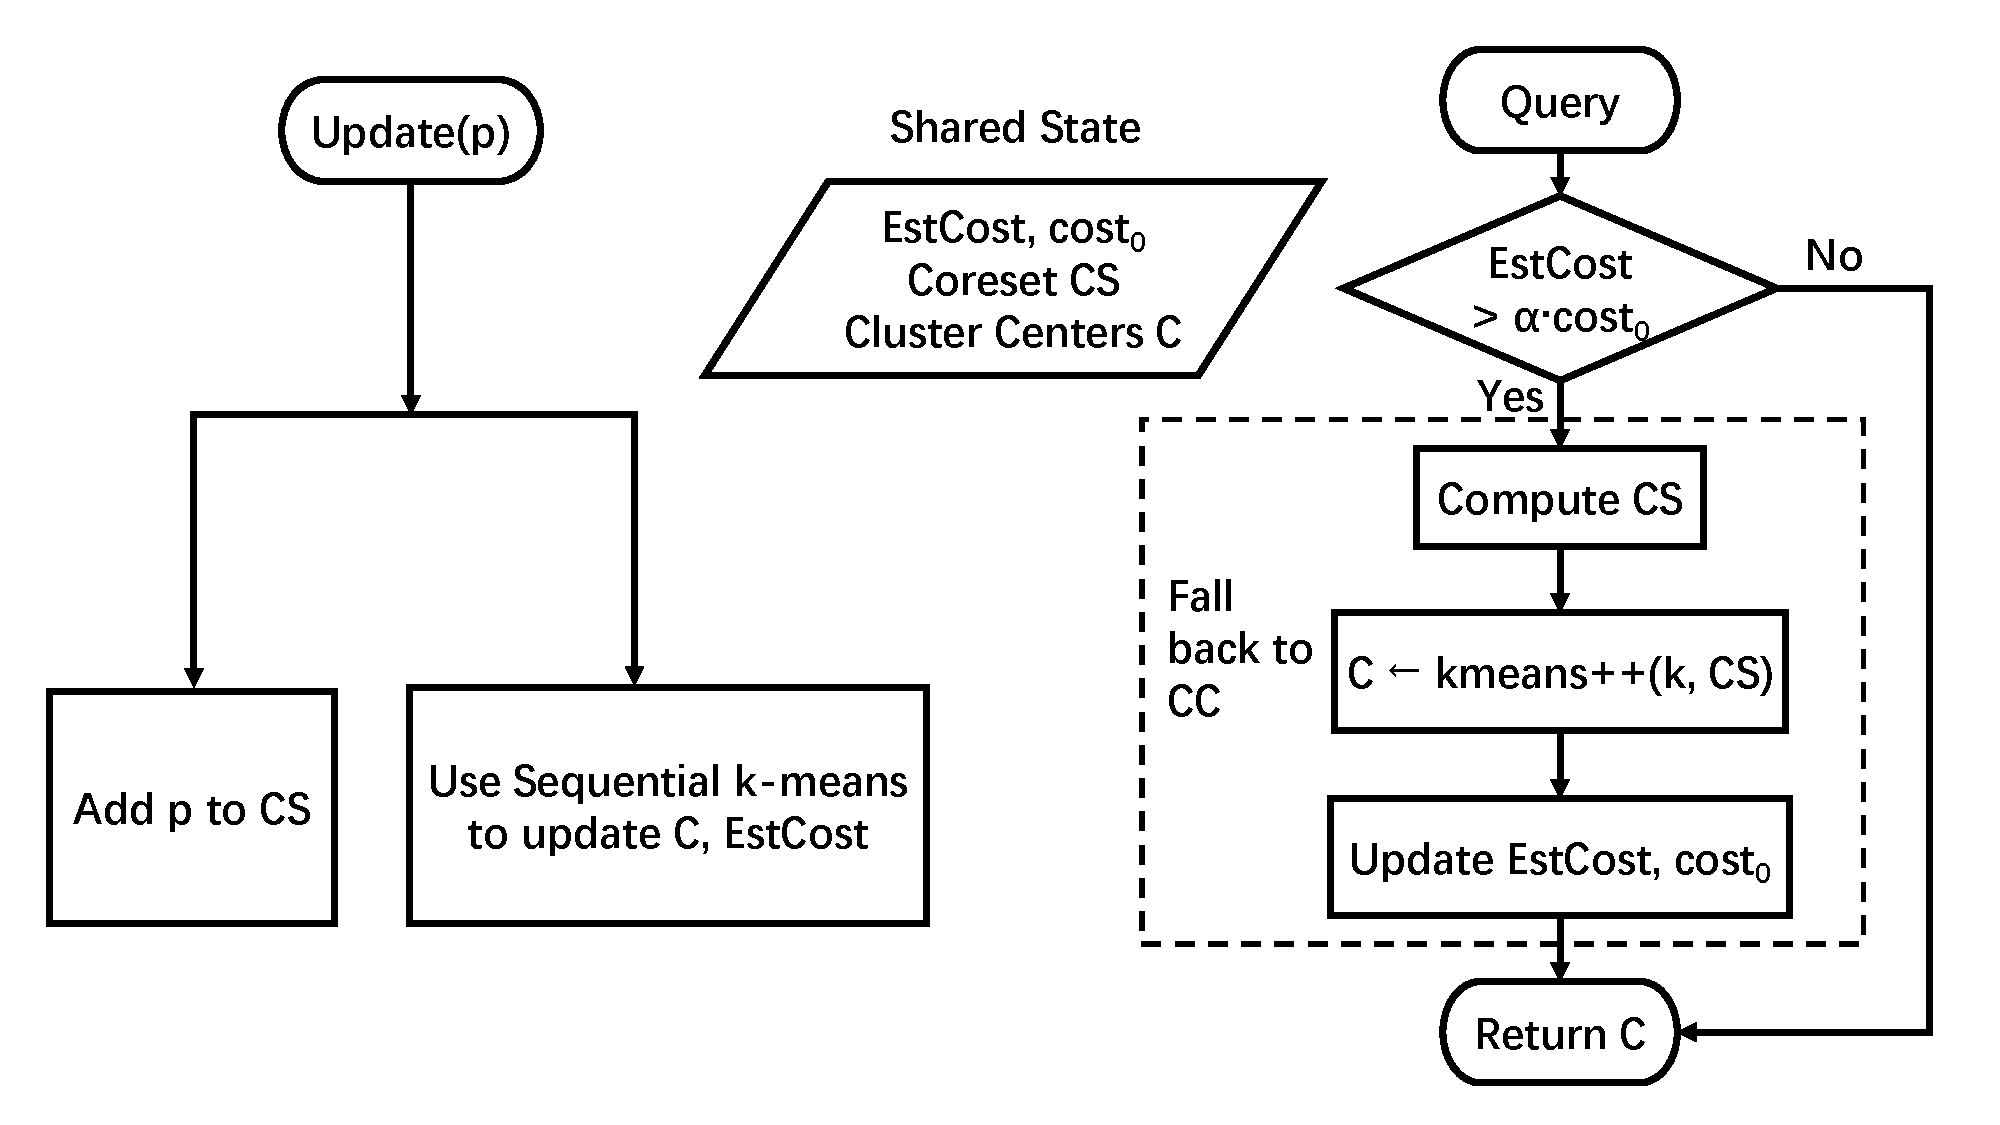
\includegraphics[width=0.49\textwidth]{figs/algo-onlinecc.pdf}
  	\caption{Illustration of Algorithm \hybrid.}
\label{fig:algo-onlinecc}
\end{figure}
%--------------------

If we break down the query runtime of the algorithms considered so far, we
observe two major components: (1)~the construction of the coreset of all points
seen so far, through merging stored coresets; and (2)~the \kmpp algorithm
applied on the resulting coreset. The focus of the algorithms discussed so far (
\cc and \rcc) is on decreasing the runtime of the first component, coreset
construction, by reducing the number of coresets to be merged at query time. But
they still have to pay the cost of the second component \kmpp, which is
substantial in itself, since the runtime of \kmpp is $O(kdm)$, where $m$ is the
size of the coreset. To make further progress, we have to reduce this
component. However, the difficulty in eliminating \kmpp at query time is that
without an approximation algorithm such as \kmpp, we have no way to guarantee
that the returned clustering is an approximation to the optimal.


This section presents an algorithm, \hybrid, which only occasionally runs \kmpp
at query time, and most of the time, uses a much cheaper method that costs
$O(1)$ to compute the clustering centers. \hybrid uses a combination of \cc and
the \seqkm algorithm~\cite{MacQueen67} (aka. Online Lloyd's algorithm) to
maintain the cluster centers quickly while also providing a guarantee on the
quality of clustering. Like \seqkm, it incrementall updates the current set of
cluster centers for each arriving point. However, while \seqkm can process
incoming points (and answer queries) extremely quickly, it cannot provide any
guarantees on the quality of answers, and in some cases, the clustering quality
can be very poor when compared with say, \kmpp. To prevent such deterioration in
clustering quality, our algorithm (1)~occasionally falls back to \cc, which is
provably accurate, and (2)~runs \seqkm so long as the clustering cost does not
get much larger than the previous time \cc was used. This ensures that our
clusters always have a provable quality with respect to the optimal.

To accomplish this, \hybrid also processes incoming points using \cc, thus
maintaining coresets of substreams of data seen so far. When a query arrives, it
typically answers them in $O(1)$ time using the centers maintained using
\seqkm. If, however, the clustering cost is significantly higher (by more than a
factor of $\alpha$ for a parameter $\alpha > 1$) than the previous time that the
algorithm fell back to \cc, then the query processing again returns to \cc to
regenerate a coreset. One difficulty in implementing this idea is that
(efficiently) maintaining an estimate of the current clustering cost is not
easy, since each change in cluster centers can affect the contribution of a
number of points to the clustering cost. To reduce the cost of maintenance, our
algorithm keeps an upper bound on the clustering cost; as we show further, this
is sufficient to give a provable guarantee on the quality of clustering. Further
details on how the upper bound on the clustering cost is maintained, and how
algorithms \seqkm and \cc interact are shown in Algorithm~\ref{algo:hybrid}, 
with a schematic illustration in Figure~\ref{fig:algo-onlinecc}.


%----------------
\begin{algorithm}[t]
\label{algo:hybrid}
\caption{The Online Coreset Cache: A hybrid of \cc and \seqkm algorithms}

\fnDef{$\hybridinit(k, \eps, \alpha)$}{
%Remember coreset approximation factor $\eps$, merge-degree $r$, and parameter $\alpha > 1$ the threshold to switch the query processing to \cc \;

\tcp{$C$ is the current set of cluster centers}
Initialize $C$ by running $\kmpp$ on set $\stream_0$ consisting of the first $O(k)$ points of the stream\;

\tcp{\fallbackcost is the clustering cost during the previous ``fallback'' to \cc; 
\estcost is an estimate of the clustering cost of $C$ on the stream so far}
\fallbackcost , \estcost $\gets$ clustering cost of $C$ on $\stream_0$\;
$Q \gets \ccinit(r,k,\eps)$\;
}

\tcp{On receiving a new point $p$ from the stream}
\fnDef{$\hybridupdate(p)$}{
	Assign $p$ to the nearest center $c_p$ in $C$  \;

    $\estcost \gets \estcost + \edist{p}{c_p}^2$ \;
	
	\tcp{Compute new centroid of $c_p$ and $p$ where $w$ is the weight of $c_p$}
	$c_p'  \gets (w \cdot c_p + p) / (w + 1)$   \; 
	Assign the position of $c_p'$ to $c_p$  \;
    Add $p$ to the current bucket $b$. If $|b|=m$, then $Q.\ccupdate(b)$ \;
}

\fnDef{$\hybridquery()$}{
	\If{$\estcost > \alpha \cdot \fallbackcost$}
	{
	     $CS \gets Q.\cccoreset() \cup b$, where $b$ is the current bucket that not yet inserted into $Q$ \;

             $C \gets \kmpp(k, CS)$   \;
             $\fallbackcost \gets \phi_C(CS)$, the \km cost of coreset $CS$ on centers $C$  \;
             $\estcost \gets \fallbackcost / (1-\eps)$   \;
	}
  \Return $C$  \;
}
\end{algorithm}
%-----------------

We state the properties of Algorithm~\hybrid in Lemma~\ref{lemma:ecost} and ~\ref{lemma:online}.
%----------------
\begin{lemma}
\label{lemma:ecost}
In Algorithm~\ref{algo:hybrid}, after observing point set $P$ from the stream, if $C$ is the current set of cluster centers, then $\estcost$ is an upper bound on $\phi_C(P)$.
\end{lemma}
%---------------
\begin{proof}
Consider the value of $\estcost$ between every two consecutive switches to \cc. Without loss of generality, suppose there is one switch happens at time $0$, let $P_0$ denote the points observed until time $0$ (including the points received at $0$). We will do induction on the number of points received after time $0$, we denote this number as $i$. Then $P_i$ is $P_0$ union the $i$ points received after time $0$. Let $\estcost (i)$ denote the cost $\estcost$ at time $i$. 

When $i$ is $0$, we compute $C$ from the coreset $CS$, from the coreset definition
\[
\fallbackcost = \phi_{C}(CS) \geq (1-\epsilon) \cdot \phi_{C}(P_0)
\] 
where $\epsilon$ is the approximation factor of coreset $CS$. So for dataset $P_0$, 
the estimation cost $\estcost(0) = \fallbackcost / (1-\eps) \geq \phi_{C}(P_0)$.

At time $i$, denote $C_i$ as the cluster centers maintained and $\estcost_i$ as the estimation of \km cost. Assume the statement is true such that $\estcost (i) > \phi_{C_i}(P_i)$. 

Consider when a new point $p$ comes, $c_p$ is the nearest center in $C_i$ to $p$. 
We compute $c_p'$, the new position of $c_p$, let $C_{i+1}$ denote the new center set 
where $C_{i+1}=C_i \setminus \{ c_p \} \cup \{c_p' \}$. 

\remove{
From the Fact~\ref{fact:ecostextension}, we know that
\[
\phi_{C_i}(S(i)) + w \edist{c_p}{c_p'}^2 + 2wD \cdot \edist{c_p}{c_p'} \geq \phi_{C_{i+1}}(S(i))
\] 
As $c_p'$ is the centroid of $c_p$ and $p$, we have
\[
\edist{p}{c_p'} < \edist{p}{c_p} = min_{c \in C_{i}} \edist{p}{c}
\]
So $c_p'$ is the nearest center in $C_{i+1}$ to $p$. Adding up together, we get:
\[
\phi_{C_i}(S(i)) + w \edist{c_p}{c_p'}^2 + 2wD \cdot \edist{c_p}{c_p'} + \edist{p}{c_p'}^2 \geq \phi_{C_{i+1}}(S(i+1))
\]
}

Based on the $\hybridupdate(p)$ in Algorithm\ref{algo:hybrid}, 
\[
\estcost (i+1) = \estcost (i) + \edist{p}{c_p}^2
\]

From the assumption of inductive step, 
\[
\estcost (i) \geq \phi_{C_i}(P_i)
\]

As $c_p'$ is the centroid of $c_p$ and $p$, we have
\[
\edist{p}{c_p} > \edist{p}{c_p'} 
\]

Because $\phi_{C_{i+1}}(P_{i+1})$ is the true cost of point set $P_{i+1}$ on centers $C_{i+1}$,
\[
\phi_{C_i}(P_i) + \edist{p}{c_p'}^2 \geq \phi_{C_{i+1}}(P_{i+1})
\] 

Adding up together, we get:
\[
\estcost (i+1) \geq \phi_{C_{i+1}}(P_{i+1})
\]
Thus the inductive step is proved.
\end{proof}
%---------------

\remove{
\begin{proof}
In Algorithm~\ref{algo:hybrid}, note that the $\estcost$ is always reset to \fallbackcost, which is equal to $\phi_C(P)$ when the query algorithm switches to \cc. Consider $\estcost$ between two consecutive switches to \cc. Without loss of generality, let the first switch happen at time $0$. Let $\stream(0)$ denote the stream observed at time $0$. We will do induction on the number of points received after time $0$, let this number be $i$. Then $\stream(i)$ is $\stream(0)$ union the $i$ points received after $0$, $\estcost_i$ is the \km cost estimation at time $i$.

When $i$ is $0$, we compute the cluster centers $C$ of coreset $CS$, from the coreset definition \ref{defn:coreset}, we have
\[
\fallbackcost = \phi_{C}(CS) \geq (1-\eps_{CS}) \cdot \phi_{C}(S(0))
\] 
where $\eps_{CS}$ is the approximation factor of coreset $CS$. So for dataset $S(0)$, $\estcost_0 = \fallbackcost / (1-\eps_{CS})$ is greater than the \km cost $\phi_{C}(S(0))$.

Let $C_i$ denote the cluster centers maintained at time $i$. Assume the statement is true that $\estcost_i > \phi_{C_i}(S(i))$. Consider a new point $p$ comes, $c_p$ is the nearest center in $C_i$ to $p$. We compute $c_p'$ which is the new position of the center $c_p$, let $C_{i+1}$ denote the new center set where $C_{i+1}=C_i \setminus \{ c_p \} \cup \{c_p' \}$. From the Fact~\ref{fact:ecostextension}, we know that
\[
\phi_{C_i}(S(i)) + w \edist{c_p}{c_p'}^2 + 2wD \cdot \edist{c_p}{c_p'} \geq \phi_{C_{i+1}}(S(i))
\] 
As $c_p'$ is the centroid of $c_p$ and $p$, we have
\[
\edist{p}{c_p'} < \edist{p}{c_p} = min_{c \in C_{i}} \edist{p}{c}
\]
So $c_p'$ is the nearest center in $C_{i+1}$ to $p$. Adding up together, we get:
\[
\phi_{C_i}(S(i)) + w \edist{c_p}{c_p'}^2 + 2wD \cdot \edist{c_p}{c_p'} + \edist{p}{c_p'}^2 \geq \phi_{C_{i+1}}(S(i+1))
\]
From the assumption $\estcost_i \geq \phi_{C_i}(S(i))$, we prove that $\estcost_{i+1} \geq \phi_{C_{i+1}}(S(i+1))$.
\end{proof}
%----------------

\begin{fact}
  \label{fact:ecostextension}
  Let $\mathcal{C}$ be the cluster centers of point set $P$, consider one of the centers $c$, denote $P_c$ as the subset of $P$ whose nearest center is $c$ in $\mathcal{C}$. Suppose $c$ moves to $c'$, then the \km cost increases at most $w \cdot \edist{c}{c'}^2 + 2w \cdot D \cdot \edist{c}{c'}$ where $w$ is the number of points in $P_c$ and $D$ is the standard deviation of cluster $P_c$. 
\end{fact}
\begin{proof}
With $c$ moves to $c'$, let $\mathcal{C}'$ be the new center set, consider the distance changed of every point to its nearest center:

\underline{Case I:}  For each point $x \in P$ but $\notin P_c$,  denote $x$'s nearest center as $e$ in $\mathcal{C}$, we have $\edist{x}{e} \geq min_{g \in C'} \edist{x}{g}$, so the \km cost of $x$ does not increase.

\underline{Case II:} For each point $x \in P_c$, we claim $\edist{x}{c'}^2$ is always the upper bound of the \km cost of $x$,
because if $x$ changes its cluster center from $c'$ to another center $e$ in $\mathcal{C}'$, then we must have $\edist{x}{e} < \edist{x}{c'}$. Based on the Triangle Inequity: 
\begin{align*}
\edist{x}{c'}^2 & \leq \left( \edist{x}{c} + \edist{c}{c'}  \right)^2 \\
					  &= \edist{x}{c}^2 + \edist{c}{c'} + 2 \cdot \edist{x}{c} \cdot \edist{c}{c'}
\end{align*}

To sum up all the \km cost increments of points in $P_c$, we get $w \cdot \edist{x}{c}^2 + 2 \cdot \edist{c}{c'} \cdot \sum_{x \in P_c} \edist{x}{c}$. As
\[
\sum_{x \in P_c} \edist{x}{c} \leq w \cdot \sqrt{\frac{ \sum_{x \in P_c} \edist{x}{c}^2}{w}} = w \cdot D
\]
where $D$ is the standard deviation of cluster $P_c$, so $w \cdot \edist{c}{c'}^2 + 2w \cdot D \cdot \edist{c}{c'}$ is the upper bound of the \km cost increment.
\end{proof}
}

%----------------
\begin{lemma}
\label{lemma:online}
When queried after observing point set $P$, the \hybrid algorithm returns a set of $k$ points $C$ whose clustering cost is within $O(\log k)$ of the optimal $k$-means clustering cost of $P$, in expectation.
\end{lemma}
%----------------

\begin{proof}
  Let $\phi^*(P)$ denote the optimal \km cost for $P$. We will show that
  $\phi_C(P) = O(\log k) \cdot \phi^*(P)$. There are two cases:

  \noindent{}\underline{Case I}: When $C$ is directly retrieved from \cc, 
  Lemma~\ref{lemma:cctree-accuracy} implies that
  $\expct{\phi_{C}(P)} \leq O(\log k) \cdot \phi^* (P)$. This case is handled
  through the correctness of \cc.

  \noindent{}\underline{Case II}:
  The query algorithm does not fall back to \cc. We first note from
  Lemma~\ref{lemma:ecost} that $\phi_C(P) \le \estcost$. Since the algorithm did
  not fall back to \cc, we have $\estcost \leq \alpha \cdot \fallbackcost$. Since
  \fallbackcost was the result of applying $\cc$ to the $P_0$ which is the point set received when last recent fall back, 
  we have from Lemma~\ref{lemma:cctree-accuracy} that
  $\fallbackcost \leq O(\log k) \cdot \phi^*(P_0)$. Since $P_0 \subseteq P$, we know
  that $\phi^*(P_0) \leq \phi^*(P)$. Putting together the above four
  inequalities, we have $\phi_C(P) = O(\log k) \cdot \phi^*(P)$.  
\end{proof}
%----------------
